%!TEX root = ./template-skripsi.tex
%-------------------------------------------------------------------------------
%                            BAB II
%               KAJIAN TEORI
%-------------------------------------------------------------------------------

\chapter{KAJIAN TEORI}                

\section{Steganografi}
	\subsection{Pengertian Steganografi}
	Menurut \textbf{Gary C. Kessler} dalam jurnalnya \emph{Steganography Hiding Data Within Data}:
	
	"Steganografi adalah ilmu menyembunyikan informasi. Tujuan steganografi adalah untuk menyembunyikan data dari pihak ketiga." \cite{kessler}.
	
	Secara umum, steganografi adalah seni untuk menyembunyikan pesan ke dalam media lain sedemikian rupa sehingga membuat orang lain tidak menyadari adanya pesan di media tersebut.
	
	\begin{figure}[H]
		\centering
		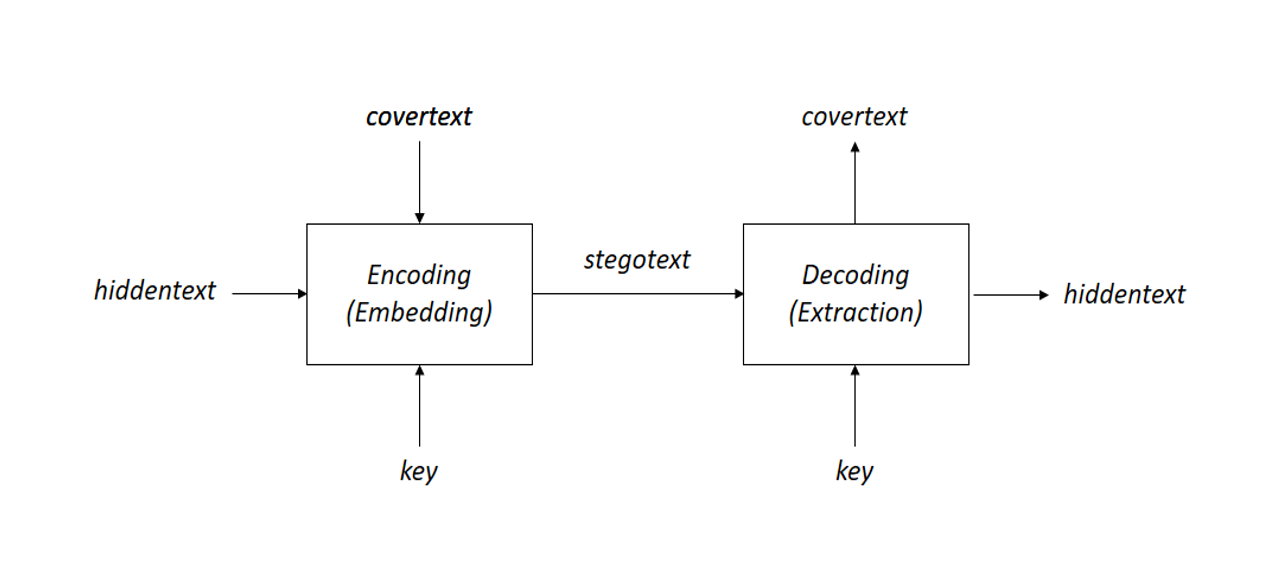
\includegraphics[width=1\textwidth]{gambar/diagram_steganografi}
		\caption{Diagram penyisipan dan ekstraksi pada pesan}
		\label{diagram_steganografi}
	\end{figure} 
	
	Istilah di dalam steganografi:
	\begin{enumerate}
		\item \emph{Covertext} merupakan media atau tempat pesan yang digunakan untuk menyembunyikan \emph{hiddentext}. \emph{Covertext} bisa berupa teks, gambar, audio, video, dll.
		\item \emph{Hiddentext}	atau biasa disebut \emph{embedded message} merupakan pesan atau informasi yang ingin disembunyikan. Contohnya bisa berupa teks, gambar, audio, video, dll.
		\item \emph{Stegotext} merupakan pesan yang sudah berisi \emph{embedded message}.
		\item \emph{Encoding} yaitu penyisipan pesan ke dalam media \emph{covertext}.
		\item \emph{Decoding} yaitu ekstraksi pesan dari \emph{stegotext}.
	\end{enumerate}
	
	Menurut \textbf{Munir}, ada kriteria yang harus diperhatikan dalam penyembunyian pesan, yaitu meliputi \emph{Imperceptible}, \emph{Fidelity}, \emph{Recovery} dan \emph{Capacity}.
	\begin{enumerate}
		\item \emph{Imperceptible}\\ 
		Keberadaan pesan rahasia tidak dapat dipersepsi secara visual atau secara audio. Jika \emph{covertext} berupa \emph{file} citra, maka \emph{stegotext} yang dihasilkan harus sukar dibedakan oleh kasat mata dengan \emph{covertext}-nya. Dan jika \emph{covertext} berupa \emph{file} audio, maka telinga tidak dapat mendeteksi perubahan yang ada pada audio \emph{stegotext}-nya. 
		\item \emph{Fidelity}\\
		Kualitas \emph{file} citra penampung tidak jauh berubah. Setelah penambahan pesan rahasia, citra hasil steganografi masih terlihat dengan baik. Pengamat tidak mengetahui kalau di dalam citra tersebut terdapat pesan rahasia.
		\item \emph{Recovery}\\
		Pesan yang disembunyikan harus dapat diekstrak kembali. Karena tujuan steganografi adalah menyembunyikan pesan atau informasi, maka jika informasi itu dibutuhkan harus dapat diambil kembali untuk dapat digunakan.
		\item \emph{Capacity}\\
		Ukuran pesan yang akan disembunyikan sedapat mungkin besar. Agar dapat memaksimalkan manfaat dari steganografi itu sendiri \cite{munir}.
	\end{enumerate}
	
	\subsection{Sejarah Steganografi}
	Seperti kriptografi, penggunaan steganografi sebetulnya telah digunakan berabad-abad yang lalu bahkan sebelum istilah steganografi itu sendiri muncul. Periode sejarah steganografi dapat dibagi menjadi:
	\begin{enumerate}
		\item Steganografi Kuno (\emph{Ancient Steganography})
			\begin{enumerate}
				\item Steganografi dengan media kepala budak
				
				Ditulis oleh \textbf{Herodatus} (485–525 BC), sejarawan Yunani pada tahun 440 BC di dalam buku: \emph{Histories of Herodatus}). Kisah perang antara kerajaan Persia dan rakyat Yunani. \textbf{Herodatus} menceritakan cara \textbf{Histaiaeus} mengirim pesan kepada \textbf{Aristagoras of Miletus} untuk melawan Persia. 
				
				Caranya adalah dengan dipilih beberapa budak. Kemudian kepala budak tersebut digunduli dan ditulis pesan dengan cara ditato. Setelah pesan dituliskan, budak harus menunggu hingga rambutnya tumbuh kembali. Setelah rambut pada kepala budak tersebut tumbuh, budak dikirim ke tempat penerima. Di sana kepala budak digunduli agar pesan dapat dibaca.
					\begin{figure}[H]
						\centering
						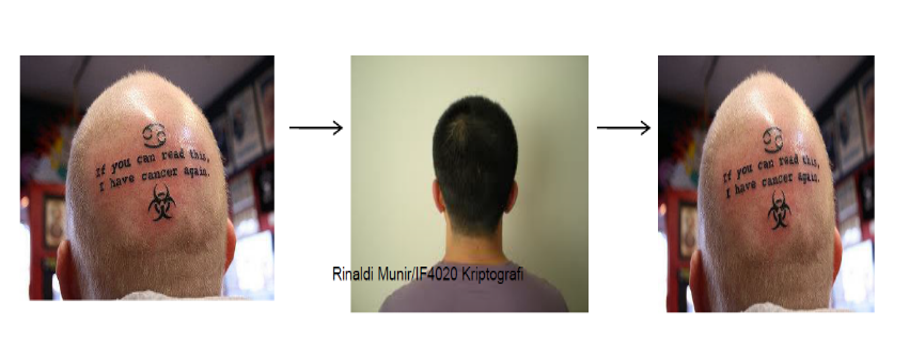
\includegraphics[width=1\textwidth]{gambar/steganografi_kepalabudak}
						\caption{Steganografi dengan media kepala budak}
						\label{steganografi_kepalabudak}
					\end{figure}
				
				\item Penggunaan tablet \emph{wax}
				
				Orang-orang Yunani kuno menulis pesan rahasia di atas kayu yang kemudian ditutup dengan lilin (\emph{wax}). Di dalam bukunya, \textbf{Heradatus} menceritakan \textbf{Demaratus} mengirim peringatan tentang serangan yang akan datang ke Yunani dengan menulis langsung pada tablet kayu yang kemudian dilapisi lilin dari lebah.
					\begin{figure}[H]
						\centering
						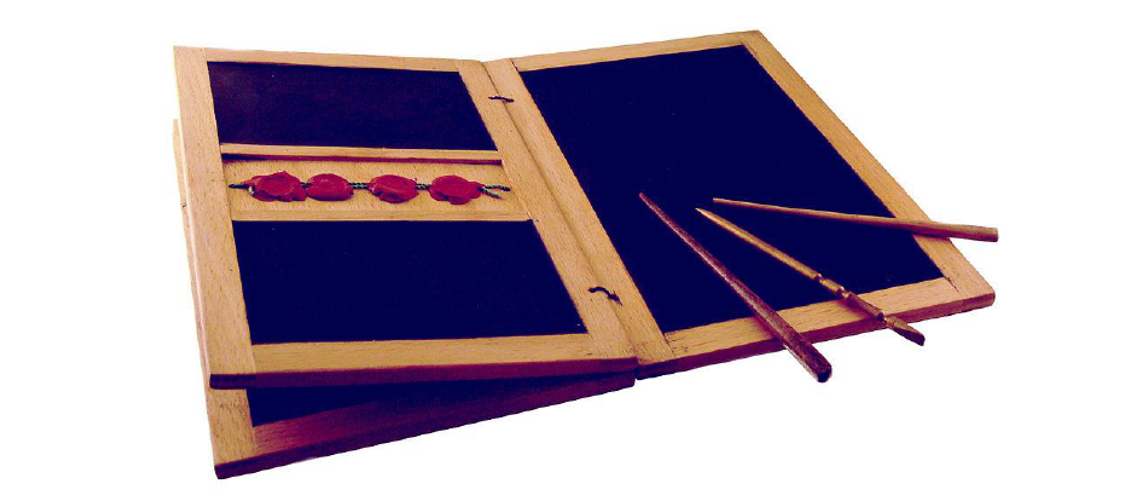
\includegraphics[width=1\textwidth]{gambar/tablet_wax}
						\caption{Tablet \emph{wax}}
						\label{tablet_wax}
					\end{figure}
					
				\item Penggunaan tinta tak-tampak (\emph{invisible ink})
				
				\textbf{Pliny the Elder} menjelaskan penggunaan tinta dari getah tanaman \emph{thithymallus}. Jika dituliskan pada kertas maka tulisan dengan tinta tersebut tidak kelihatan, tetapi bila kertas dipanaskan berubah menjadi gelap/coklat.
				
				\item Penggunaan kain sutra dan lilin
				
				Orang Cina kuno menulis catatan pada potongan-potongan kecil sutra yang kemudian digumpalkan menjadi bola kecil dan dilapisi lilin. Selanjutnya bola kecil tersebut ditelan oleh si pembawa pesan. Pesan dibaca setelah bola kecil dikeluarkan dari perut si pembawa pesan.			
			\end{enumerate}
		\item Steganografi Zaman Renaisans (\emph{Renaissance Steganography})
		
		Tahun 1499, \textbf{Johannes Trithemius} menulis buku \emph{Steganographia}, yang menceritakan tentang metode steganografi berbasis karakter. Selanjutnya tahun 1518 dia menulis buku tentang steganografi dan kriptografi berjudul \emph{Polygraphiae}. \textbf{Giovanni Battista Porta} menggambarkan cara menyembunyikan pesan di dalam telur rebus. Caranya, pesan ditulis pada kulit telur yang dibuat dari tinta khusus yang dibuat dengan satu ons tawas dan setengah liter cuka. Prinsipnya penyembunyiannya adalah tinta tersebut akan menembus kulit telur yang berpori, tanpa meninggalkan jejak yang terlihat. Tulisan dari tinta akan membekas pada permukaan isi telur yang telah mengeras (karena sudah direbus sebelumnya). Pesan dibaca dengan membuang kulit telur.
		
		\item Steganografi Zaman Perang Dunia (\emph{World War Steganography})
		
		\begin{figure}[H]
			\centering
			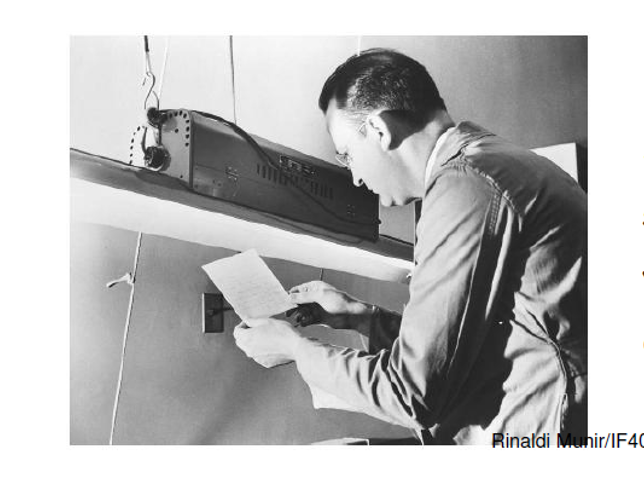
\includegraphics[width=1\textwidth]{gambar/steganografi_perangdunia}
			\caption{Steganografi zaman perang dunia}
			\label{steganografi_perangdunia}
		\end{figure}
	
		Selama terjadinya Perang Dunia ke-2, tinta yang tidak tampak (\emph{invisible ink}) telah digunakan untuk menulis informasi pada lembaran kertas sehingga saat kertas tersebut jatuh di tangan pihak lain hanya akan tampak seperti lembaran kertas kosong biasa. Cairan seperti air kencing (\emph{urine}), susu, vinegar, dan jus buah digunakan sebagai media penulisan sebab bila salah satu elemen tersebut dipanaskan, tulisan akan menggelap dan tampak melalui mata manusia \cite{munir}.
		
		\item Steganografi \emph{Digital}
		
		Sejalan dengan perkembangan maka konsep awal steganografi diimplementasikan pula dalam dunia komputer, yang kemudian dikenal dengan istilah steganografi \emph{digital}. Dalam hal ini, steganografi \emph{digital} memiliki dua properti dasar yaitu media penampung (\emph{cover data} atau \emph{data carrier}) dan data \emph{digital} yang akan disisipkan (\emph{secret data}), dimana media penampung dan data \emph{digital} yang akan disisipkan dapat berupa \emph{file} multimedia (teks/dokumen, citra, audio maupun video). Terdapat dua tahapan umum dalam steganografi \emph{digital}, yaitu proses \emph{embedding} atau \emph{encoding} (penyisipan) dan proses \emph{extracting} atau \emph{decoding} (pemekaran atau pengungkapan kembali (\emph{reveal})). Hasil yang didapat setelah proses \emph{embedding} atau \emph{encoding} disebut \emph{stego object} (apabila media penampung hanya berupa data citra maka disebut \emph{stego image}) \cite{prayudi}.
	\end{enumerate}

	\subsection{Metode Steganografi}
	Berdasarkan ranah operasinya, metode-metode steganografi dapat dibagi menjadi dua kelompok:
	\begin{enumerate}
		\item \emph{Spatial (time) domain methods}\\
		Memodifikasi langsung nilai byte dari \emph{cover-object} (nilai \emph{byte} dapat merepresentasikan intensitas/warna \emph{pixel} atau amplitudo). Contoh: Metode modifikasi LSB
		
		\item \emph{Tranform domain methods}\\
		Memodifikasi hasil transformasi sinyal dalam ranah transform (hasil transformasi dari ranah spasial ke ranah lain (misalnya ranah frekuensi). Contoh: Metode \emph{Spread Spectrum} \cite{munir}.
		
	\end{enumerate}

	Ada empat jenis metode steganografi:
	\begin{enumerate}
		\item \emph{Least Significant Bit Insertion} (LSB)\\
		Metode yang digunakan untuk menyembunyikan pesan pada media \emph{digital} tersebut berbeda-beda. Contohnya, pada berkas \emph{image} pesan dapat disembunyikan dengan menggunakan cara menyisipkannya pada bit rendah atau bit yang paling kanan (LSB) pada data \emph{pixel} yang menyusun \emph{file} tersebut. Pada berkas \emph{bitmap} 24 bit, setiap \emph{pixel} (titik) pada gambar tersebut terdiri dari susunan tiga warna \emph{Red}, \emph{Green} dan \emph{Blue} (RGB) yang masing-masing disusun oleh bilangan 8 bit (\emph{byte}) dari 0 sampai 255 atau dengan format biner 00000000 sampai 11111111. Dengan demikian, pada setiap \emph{pixel} berkas \emph{bitmap} 24 bit kita dapat menyisipkan 3 bit data. 
		\item \emph{Algorithms and Transformation}\\
		\emph{Algoritma compression} adalah metode steganografi dengan menyembunyikan data dalam fungsi matematika. Dua fungsi tersebut adalah \emph{Discrete Cosine Transformation} (DCT) dan \emph{Wavelet Transformation}. Fungsi DCT dan \emph{Wavelet} yaitu mentransformasi data dari satu tempat (\emph{domain}) ke tempat (\emph{domain}) yang lain. Fungsi DCT yaitu mentransformasi data dari tempat \emph{spatial} (\emph{spatial domain}) ke tempat frekuensi (\emph{frequency domain}).
		\item \emph{Redundant Pattern Encoding}\\
		\emph{Redundant Pattern Encoding} adalah menggambar pesan kecil pada kebanyakan gambar. Keuntungan dari metode ini adalah dapat bertahan dari \emph{cropping} (kegagalan). Kerugiannya yaitu tidak dapat menggambar pesan yang lebih besar.
		\item \emph{Spread Spectrum Method}\\
		\emph{Spread Spectrum} steganografi terpencar-pencar sebagai pesan yang diacak (\emph{encrypted}) melalui gambar (tidak seperti dalam LSB). Untuk membaca suatu pesan, penerima memerlukan algoritma yaitu \emph{crypto-key} dan \emph{stego-key}. Metode ini juga masih mudah diserang yaitu penghancuran atau pengrusakan dari kompresi dan proses \emph{image} (gambar) \cite{wikipedia1}.
	\end{enumerate}

	Metode LSB dan \emph{Spread Spectrum} adalah dua metode yang sering digunakan dalam melakukan steganografi. Selain karena metodenya yang sederhana, proses \emph{encoding} dan \emph{decoding} dari kedua metode tersebut juga \emph{relative} cepat\cite{pavani}. Tetapi LSB memiliki proses \emph{encoding} dan \emph{decoding} yang lebih cepat dari metode \emph{Spread Spectrum} karena proses metode \emph{Spread Spectrum} harus melalui proses XOR antara pesan dan kata kunci, sedangkan LSB langsung menyisipkan pesan ke dalam gambar \cite{pakereng}.
	
	\begin{figure}[H]
		\centering
		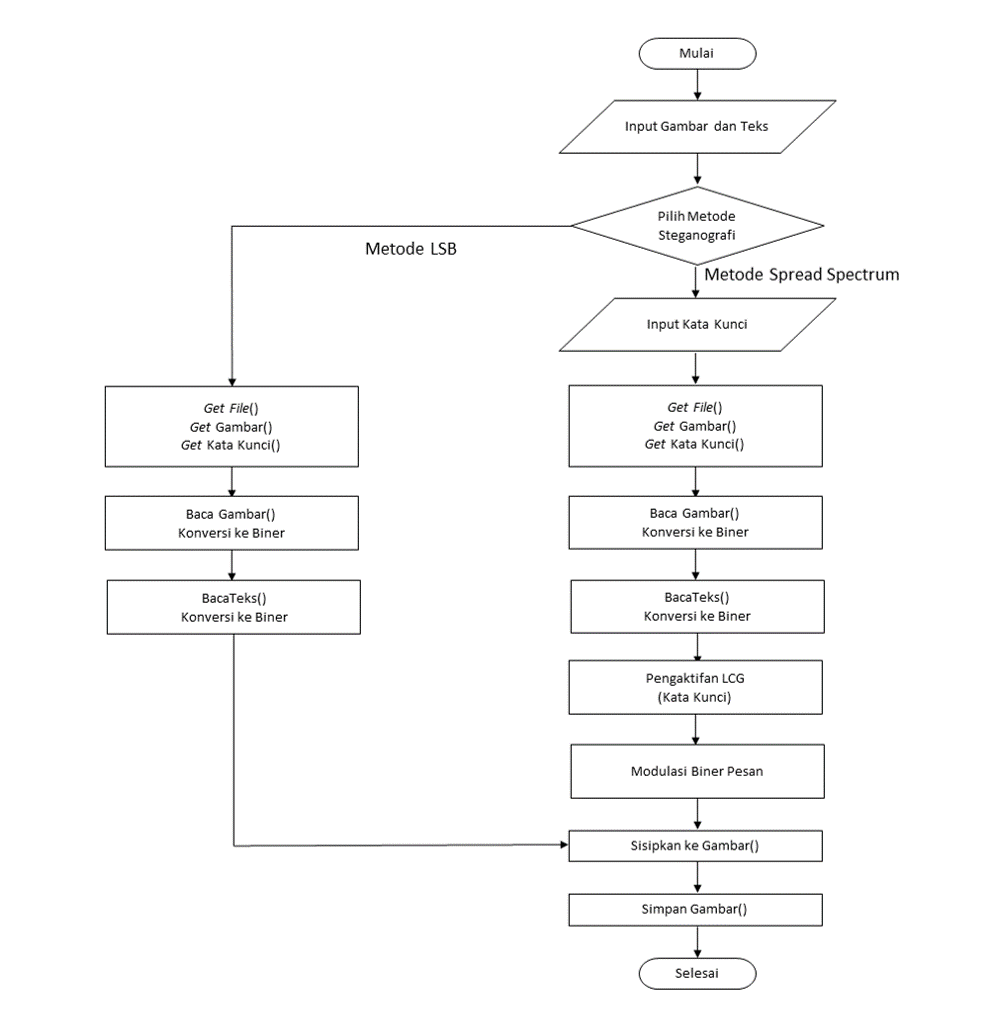
\includegraphics[width=1\textwidth]{gambar/spreadlsb}
		\caption{\emph{Flowchart Encoding} LSB dan \emph{Spread Spectrum}}
		\label{spreadlsb}
	\end{figure}
	

\section{Perbedaan Steganografi dan Kriptografi}
Steganografi dan kriptografi mempunyai prinsip kerja yang berbeda, meskipun keduanya mempunyai hubungan yang dekat dalam dunia keamanan data. Pada kriptografi menghasilkan sebuah \emph{chipertext} dimana dengan itu seolah-olah dengan sengaja menunjukkan kepada orang lain bahwa ada sesuatu di dalamnya, namun tidak dapat diketahui maknanya. Namun dengan bentuk \emph{chiper}-nya, justru akan membuat data tersebut terancam oleh usaha-usaha yang dilakukan oleh orang lain untuk dapat membongkarnya dengan tujuan dan atau alasan apapun.
\begin{figure}[H]
	\centering
	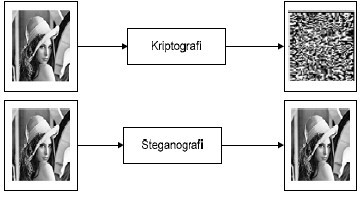
\includegraphics[width=1\textwidth]{gambar/perbedaan_kripsteg}
	\caption{Perbedaan Kriptografi dan Steganografi}
	\label{perbedaan_kripsteg}
\end{figure}

Steganografi dan kriptografi merupakan seni dan teknik yang dapat digunakan untuk melakukan pengamanan data \emph{digital}. Namun keduanya tidaklah sama. Pada kriptografi, suatu data \emph{digital} diamankan dengan cara mengenkripsi data tersebut dan menghasilkan sebuah data yang berupa sandi, secara visual data tersebut masih dapat terlihat atau diketahui, hanya saja data tersebut menjadi tidak dapat dimengerti. Berbeda dengan steganografi yang tujuannya adalah menyembunyikan data ke dalam sebuah media yang lain, sehingga data tersebut tidak terlihat \cite{setiana}.

\section{LSB (\emph{Least Significant Bit})}
Penyembunyian data dilakukan dengan mengganti bit-bit data di dalam segmen citra dengan bit-bit rahasia. Pada susunan bit di dalam sebuah \emph{byte} (1 \emph{byte}= 8 bit), ada bit yang paling berarti (\emph{most significant bit} atau MSB) dan bit yang paling kurang berarti (\emph{least significant bit} atau LSB). LSB merupakan salah satu metode yang paling sederhanaa dalam steganografi. Bit yang cocok untuk diganti adalah bit LSB, sebab perubahan tersebut hanya mengubah nilai \emph{byte} satu lebih tinggi atau satu lebih rendah dari nilai sebelumnya \cite{munir}.

Pada \emph{file bitmap} 24 bit, setiap bit masing-masing memiliki komponen \emph{Red, Green,} dan \emph{Blue} (RGB), sehingga dapat menyimpan 3 bit pada setiap \emph{pixel}-nya. Pada gambar 800x600 \emph{pixel} dapat digunakan untuk menyembunyikan 1.440.000 bit (180.000 \emph{Byte}) data rahasia. Sebagai contoh diambil 3 \emph{pixel} dari \emph{file bitmap} 24 bit yang akan disisipkan pesan atau data rahasia karakter "A":
\begin{figure}[H]
	\centering
	(00001000 00101011 11011100)\\
	(11100000 11000100 00010101)\\
	(00010011 10101010 01100011)\\
\end{figure}

Karakter "A" mempunyai nilai biner 01000001, maka bit hasil penyisipannya adalah:
\begin{figure}[H]
	\centering
	(00001000 00101011 11011100)\\
	(11100000 11000100 0001010\textbf{0})\\
	(0001001\textbf{0} 1010101\textbf{1} 01100011\\
\end{figure}

Bit-bit yang nilainya berganti ada 3 dalam 8 \emph{Byte} yang digunakan. Contoh lainnya adalah diambil 8 pixel dari sebuah gambar, maka data rahasia yang dapat dimasukkan adalah 1 kata, contohnya adalah "ADA"
\begin{figure}[H]
	\centering
	(10011011 01100100 01010000)\\
	(10010011 01010101 01001000)\\
	(10011010 01010111 01001110)\\
	(10011010 01010101 01010000)\\
	(10001000 01000001 00111111)\\
	(01101001 00100010 00110100)\\
	(01101101 00100111 00110010)\\
	(01111001 00110011 00110101)\\
\end{figure}

Kata "ADA" mempunyai biner A = 01000001, D = 01000100, maka bit hasil penyisipannya adalah:
\begin{figure}[H]
	\centering
	(1001101\textbf{0} 0110010\textbf{1} 01010000)\\
	(1001001\textbf{0} 0101010\textbf{0} 01001000)\\
	(10011010 01010111 01001110)\\
	(1001101\textbf{1} 0101010\textbf{0} 01010000)\\
	(10001000 01000001 0011111\textbf{0})\\
	(0110100\textbf{0} 00100010 0011010\textbf{1})\\
	(0110110\textbf{0} 0010011\textbf{0} 00110010)\\
	(0111100\textbf{0} 0011001\textbf{0} 00110101)\\
\end{figure}

Bit-bit yang nilainya berganti ada 13 dalam 24 \emph{Byte} yang digunakan. Secara rata-rata, LSB hanya menggunakan setengah dari bit dalam gambar yang perlu dimodifikasi untuk menyembunyikan pesan rahasia. Perubahan ini tidak dapat dirasakan oleh mata manusia, dan pesan berhasil disembunyikan \cite{elgabar2}.

\section{ASCII}
ASCII adalah singkatan dari \emph{American Standard Code for Information Interchange}. Komputer hanya dapat memahami angka, jadi kode ASCII adalah representasi numerik dari karakter seperti 'a' atau '@' atau karakter lainnya. Kode ASCII memiliki komposisi bilangan biner sebanyak 8 bit. Dimulai dari 00000000 hingga 11111111. Total kombinasi yang dihasilkan ASCII sebanyak 256, dimulai dari kode 0 hingga 255 dalam sistem bilangan desimal. \cite{ascii}
\begin{table}[H]
	\centering
	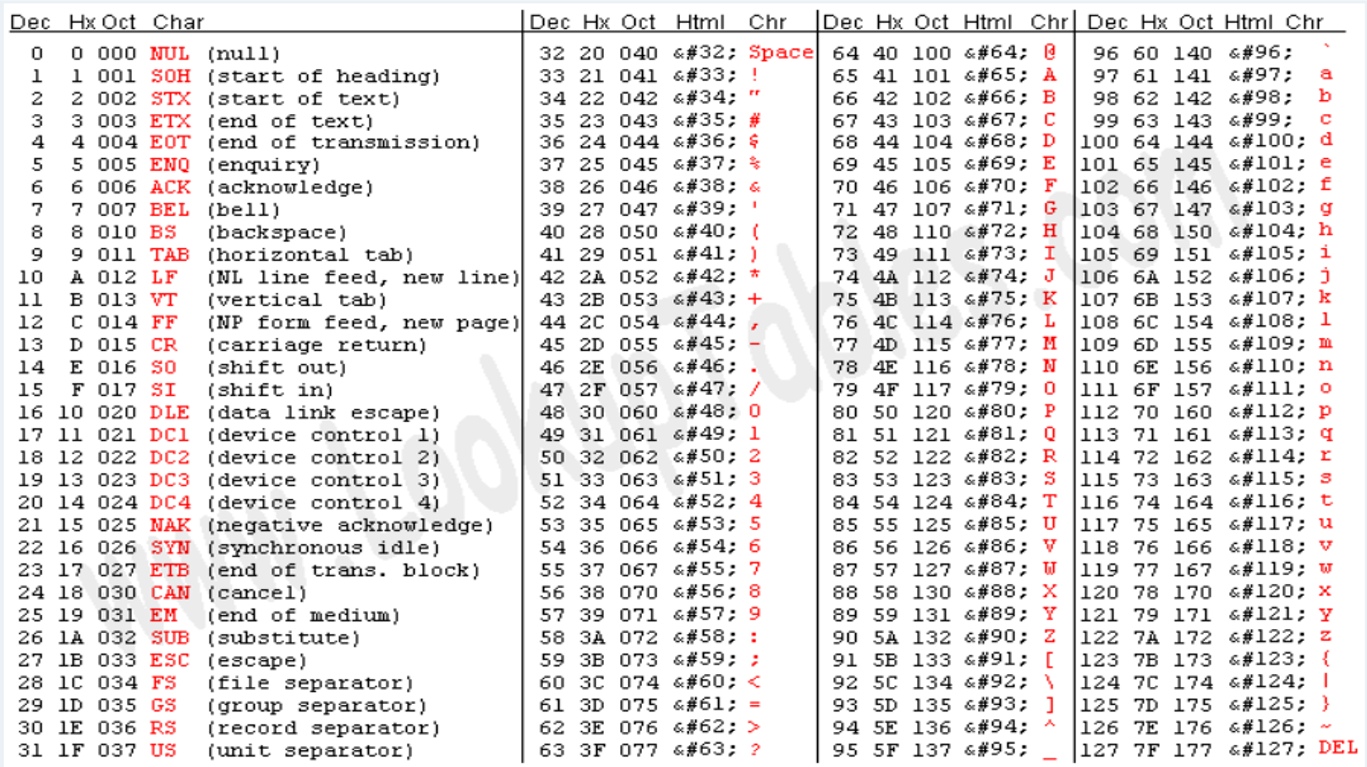
\includegraphics[width=1.0\textwidth]{gambar/table_ascii}
	\caption{Tabel ASCII}
	\label{tabel_ascii}
\end{table}

\section{Citra \emph{Digital}}
	\subsection{Pengertian Citra \emph{Digital}}
	Citra atau gambar dapat didefinisikan sebagai sebuah fungsi dua dimensi, f(x,y), x dan y adalah koordinat bidang datar; dan harga fungsi f di setiap pasangan koordinat (x,y) disebut intensitas atau level keabuan (\emph{grey level}) dari gambar di titik itu \cite{hermawati}. Citra ada 2 macam, yaitu:
	\begin{enumerate}
		\item Citra kontinu, yaitu citra yang dihasilkan dari sistem optik yang menerima sinyal analog, misal: mata manusia dan kamera analog.
		\item Citra diskrit, yaitu citra yang dihasilkan melalui proses digitalisasi terhadap citra kontinu.
	\end{enumerate}
	
	Agar dapat diolah dengan komputer, maka suatu citra harus direpresentasikan secara \emph{numeric} dengan nilai-nilai diskrit. Representasi citra dari fungsi kontinyu menjadi nilai-nilai diskrit disebut digitalisasi, dan citra yang dihasilkan disebut citra \emph{digital}.
	
	Ada 3 bidang studi utama yang menangani pengolahan data atau informasi berbentuk gambar atau citra, yaitu:
	\begin{enumerate}
		\item Grafika Komputer (\emph{Computer Graphics})
		\item Pengolahan Citra (\emph{Image Processing})
		\item Pengenalan Pola (\emph{Pattern Recognition})
	\end{enumerate}
	
	\subsection{Pengolahan Citra (\emph{Image Processing})}
	Pengolahan citra adalah pemrosesan citra, khususnya dengan menggunakan komputer, menjadi citra yang kualitasnya lebih baik. Pengolahan Citra bertujuan memperbaiki kualitas citra agar mudah diinterpretasi oleh manusia atau mesin (dalam hal ini komputer). Teknik-teknik pengolahan citra mentransformasikan citra menjadi citra lain. Jadi, masukannya adalah citra dan keluarannya juga citra, namun citra keluaran mempunyai kualitas lebih baik daripada citra masukan \cite{munir04}
	
	\subsection{Format \emph{File} pada Citra \emph{Digital}}
		\begin{enumerate}
			\item BMP\\
			BMP adalah singkatan dari \emph{Bitmap} yang dahulu dikembangkan oleh MICROSOFT. \emph{Bitmap} dapat menyimpan data warna untuk masing-masing \emph{pixel} dalam gambar tanpa kompresi apapun. Format ini dapat digunakan untuk menyembunyikan data tanpa menaikkan kecurigaan pada mata manusia. Gambar yang dihasilkan tanpa kompresi dan format \emph{lossless} yang merupakan salah satu faktor penting. Ekstensi yang digunakan dalam \emph{file} ini adalah .bmp \cite{gautam}.
			\item JPEG\\
			Istilah JPEG sebenarnya adalah singkatan dari pengembangnya, yaitu \emph{Joint Photographic Experts Group}. Gambar JPEG tidak terbatas pada sejumlah warna tertentu. Oleh karena itu, format JPEG paling baik untuk mengompresi gambar foto. Gambar dengan format JPEG dapat berisi data gambar beresolusi tinggi berwarna-warni, itu adalah format \emph{lossy}, yang berarti beberapa kualitas hilang ketika gambar dikompresi. Jika gambar terlalu banyak dikompres, grafiknya menjadi seperti "tidak berwarna" dan sebagian detailnya hilang. Ekstensi yang digunakan dalam \emph{file} ini adalah .jpeg \cite{elgabar}.
			\item GIF\\
			GIF adalah singkatan dari \emph{Graphics Interchange Format} yang dikembangkan oleh COMPUSERVICE. GIF digunakan untuk tujuan menyimpan beberapa gambar \emph{bitmap} dalam satu \emph{file} gambar. GIF sering digunakan untuk menyimpan grafik multi-bit dan data gambar. GIF tidak terkait dengan aplikasi perangkat lunak tertentu tetapi dirancang untuk memudahkan pertukaran dan tampilan data gambar yang tersimpan di lokal atau sistem komputer jarak jauh. GIF digunakan juga karena menerapkan metode kompresi \emph{lossless}. Ekstensi yang digunakan dalam \emph{file} ini adalah .gif \cite{elgabar2}.
			\item TIFF\\
			TIFF adalah singkatan dari \emph{Taged Image Format File}. TIFF dikembangkan oleh ADOBE dan digunakan untuk grafis berkualitas tinggi dengan kompresi \emph{lossless}. Format \emph{file} ini memiliki transparansi dan pilihan warna terindeks untuk menanamkan pesan rahasia di atasnya. TIFF mendukung properti RGB dan \emph{GRAYSCALE} dan digunakan untuk HD \emph{Imaging}. Ini adalah salah satu format \emph{file} paling serbaguna di antara semua format yang tersedia. Ekstensi yang digunakan dalam format \emph{file} ini adalah .tiff \cite{gautam}.
			\item PNG\\
			PNG adalah singkatan dari \emph{Portable Network Graphics} yang dikembangkan oleh PNG \emph{Development Group}. PNG mampu menyembunyikan pesan yang besar di dalamnya. Format \emph{file} ini diciptakan untuk meningkatkan format \emph{file} gambar GIF menghilangkan batasan 256 warna tetapi tidak mendukung animasi. Dan PNG menggunakan kompresi data \emph{lossless}. Ekstensi yang digunakan dalam format \emph{file} ini adalah .png \cite{gautam}.
		\end{enumerate}
	Perbedaan komponen antara masing-masing format \emph{file} citra \emph{digital} dapat dilihat pada Tabel \ref{tabel_perbedaan}. 
	\begin{table}[H]
		\centering
		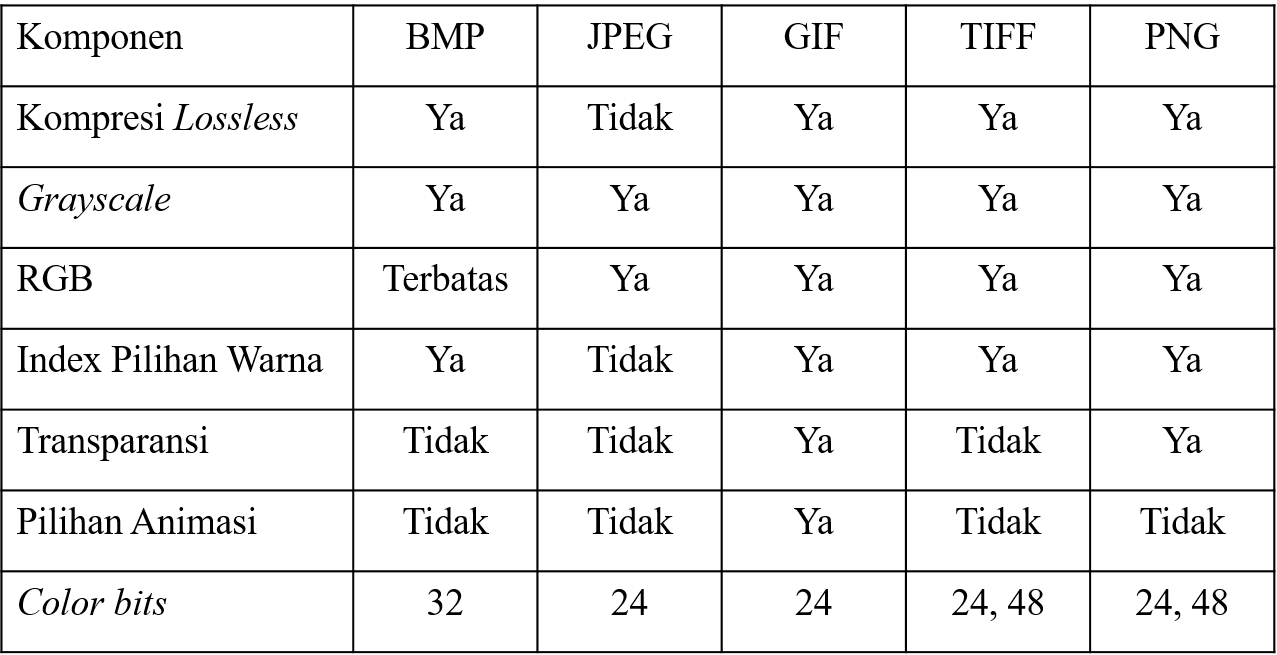
\includegraphics[width=0.8\textwidth]{gambar/table_perbedaan}
		\caption{Perbedaan \emph{file} citra \emph{digital}}
		\label{tabel_perbedaan}
	\end{table}


% Baris ini digunakan untuk membantu dalam melakukan sitasi
% Karena diapit dengan comment, maka baris ini akan diabaikan
% oleh compiler LaTeX.
\begin{comment}
bibliography{daftar-pustaka}
\end{comment}
